\section{Todos-para-Todos (\textit{All-to-All})}

No padrão \textit{todos-para-todos}, não há hierarquia nem sequência predefinida:
todos os agentes podem se comunicar diretamente com todos os demais a qualquer
momento. A comunicação ocorre em um espaço compartilhado --- análogo a uma sala de
conferência virtual ---, e cada mensagem enviada por um agente é adicionada ao
contexto dos demais participantes. A Figura~\ref{fig:alltoall} ilustra esse padrão.

\begin{figure}[ht]
\centering
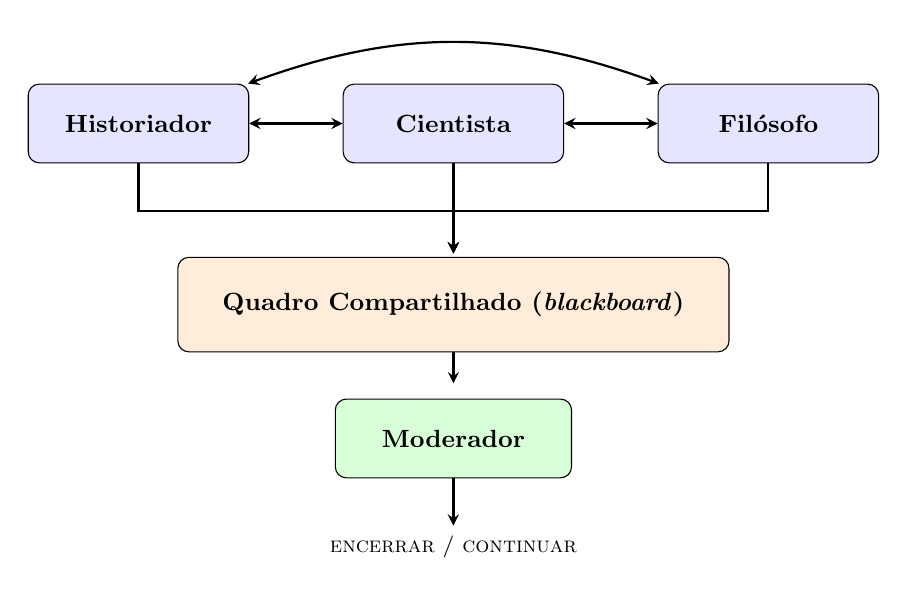
\begin{tikzpicture}[
    agent/.style={
        draw, rounded corners=4pt,
        minimum width=2.8cm, minimum height=1cm,
        fill=blue!10, font=\small\bfseries
    },
    blackboard/.style={
        draw, rounded corners=4pt,
        minimum width=7cm, minimum height=1.2cm,
        fill=orange!15, font=\small\bfseries
    },
    moderator/.style={
        draw, rounded corners=4pt,
        minimum width=3cm, minimum height=1cm,
        fill=green!15, font=\small\bfseries
    },
    arr/.style={-stealth, thick},
    biarr/.style={stealth-stealth, thick}
]

% Agentes no topo
\node[agent] (hist) at (-4, 3)   {Historiador};
\node[agent] (cien) at ( 0, 3)   {Cientista};
\node[agent] (filo) at ( 4, 3)   {Filósofo};

% Setas bidirecionais entre agentes (via quadro)
\draw[biarr] (hist) -- (cien);
\draw[biarr] (cien) -- (filo);
\draw[biarr] (hist) to[bend left=20] (filo);

% Setas dos agentes para o quadro
\draw[arr] (hist.south) -- ++(0,-0.6) -| (0, 1.35);
\draw[arr] (cien.south) -- (0, 1.35);
\draw[arr] (filo.south) -- ++(0,-0.6) -| (0, 1.35);

% Quadro compartilhado
\node[blackboard] (quadro) at (0, 0.7)
    {Quadro Compartilhado (\textit{blackboard})};

% Seta do quadro para o moderador
\draw[arr] (quadro.south) -- (0,-0.3);

% Moderador
\node[moderator] (mod) at (0,-1)   {Moderador};

% Rótulo de saída do moderador
\draw[arr] (mod.south) -- ++(0,-0.6)
    node[below, font=\footnotesize, align=center]
    {\textsc{encerrar} / \textsc{continuar}};

\end{tikzpicture}
\caption{Padrão \textit{todos-para-todos}: agentes se comunicam via quadro compartilhado; o moderador decide quando encerrar.}
\label{fig:alltoall}
\end{figure}

Na implementação, cada agente é informado da existência dos demais e pode contribuir
a qualquer momento. As contribuições são incorporadas ao quadro compartilhado, que
funciona como o contexto coletivo da discussão --- inspirado nos modelos de
\textit{blackboard} da inteligência artificial clássica, nos quais diferentes módulos
de conhecimento leem e escrevem em um espaço comum. O sistema encerra quando um
agente designado --- o moderador --- julga o resultado coletivo satisfatório.

O Código~\ref{lst:alltoall} apresenta uma implementação didática desse padrão. Três
especialistas (Historiador, Cientista e Filósofo) debatem um tema proposto. A cada
rodada, todos leem o quadro inteiro e contribuem em paralelo; o moderador avalia se
perspectivas suficientes foram apresentadas e decide pela continuação ou encerramento.

\begin{lstlisting}[
    language=Python,
    caption={Padrão \textit{todos-para-todos}: debate multiagente com quadro compartilhado.},
    label={lst:alltoall}
]
import asyncio
from agenticblocks.blocks.llm.agent import LLMAgentBlock, AgentInput

MODEL = "ollama/mistral-nemo:latest"
MAX_RODADAS = 3


def formatar_quadro(quadro: list[str]) -> str:
    return "\n".join(f"[{i+1}] {msg}" for i, msg in enumerate(quadro))


async def main():
    historiador = LLMAgentBlock(
        name="historiador",
        system_prompt=(
            "Você é um historiador. Leia o quadro compartilhado e contribua "
            "com 2-3 frases sobre a perspectiva histórica do tema. "
            "Responda SOMENTE com sua contribuição, sem prefácio."
        ),
        model=MODEL, max_iteration=0,
    )

    cientista = LLMAgentBlock(
        name="cientista",
        system_prompt=(
            "Você é um cientista. Leia o quadro compartilhado e contribua "
            "com 2-3 frases sobre a perspectiva científica do tema. "
            "Responda SOMENTE com sua contribuição, sem prefácio."
        ),
        model=MODEL, max_iteration=0,
    )

    filosofo = LLMAgentBlock(
        name="filósofo",
        system_prompt=(
            "Você é um filósofo. Leia o quadro compartilhado e contribua "
            "com 2-3 frases sobre a perspectiva filosófica do tema. "
            "Responda SOMENTE com sua contribuição, sem prefácio."
        ),
        model=MODEL, max_iteration=0,
    )

    moderador = LLMAgentBlock(
        name="moderador",
        system_prompt=(
            "Você é o moderador da discussão. Avalie o quadro compartilhado. "
            "Se houver contribuições de pelo menos três perspectivas distintas, "
            "responda com 'ENCERRAR' seguido de um resumo de 3 linhas. "
            "Caso contrário, responda apenas 'CONTINUAR'."
        ),
        model=MODEL, max_iteration=0,
    )

    agentes = [historiador, cientista, filosofo]
    nomes   = ["Historiador", "Cientista", "Filósofo"]

    tema  = "O impacto da inteligência artificial na sociedade humana."
    quadro: list[str] = [f"TEMA: {tema}"]

    for rodada in range(1, MAX_RODADAS + 1):
        # Todos os agentes leem o quadro e contribuem em paralelo
        contexto  = f"Quadro compartilhado:\n{formatar_quadro(quadro)}"
        respostas = await asyncio.gather(
            *[agente.run(AgentInput(prompt=contexto)) for agente in agentes]
        )

        # Cada contribuição é adicionada ao quadro, visível a todos
        for nome, resposta in zip(nomes, respostas):
            quadro.append(f"[{nome}] {resposta.response}")

        # O moderador avalia se a discussão está completa
        avaliacao = await moderador.run(
            AgentInput(prompt=f"Quadro compartilhado:\n{formatar_quadro(quadro)}")
        )
        if "ENCERRAR" in avaliacao.response.upper():
            break


if __name__ == "__main__":
    asyncio.run(main())
\end{lstlisting}

O ponto central da implementação é a função \texttt{formatar\_quadro} (linha~3), que
serializa o estado atual do quadro em texto simples. Esse texto é passado como
\texttt{prompt} para cada agente, garantindo que todos partam do mesmo contexto antes
de contribuir.

Na linha~55, \texttt{asyncio.gather} dispara todos os agentes \emph{simultaneamente},
reproduzindo a dinâmica paralela do padrão: nenhum especialista espera a resposta dos
outros para formular a sua. As contribuições chegam de forma assíncrona e são
ordenadas apenas no momento da inserção no quadro (linhas~60--61).

O moderador (linhas~63--65) opera de forma independente dos especialistas: ele lê o
mesmo quadro e emite um veredicto binário. Essa separação entre \emph{produtores de
conhecimento} e \emph{árbitro de encerramento} é característica do padrão
\textit{todos-para-todos} e permite que a condição de parada seja tão simples ou
sofisticada quanto o problema exigir --- desde uma contagem de contribuições até uma
análise semântica profunda realizada pelo próprio LLM.
